\section{Future forecasting}
\label{sec:forecasting}

The future is often uncertain. As shown in \Cref{fig:narration_chart}, a sequence of steps can lead to multiple possible scenarios. Anticipation models are trained on objectives that require the discovery of domain-specific knowledge to address future anticipation challenges. We discuss methods for anticipating categorical semantics in \Cref{sec:forecasting::anticipation}. We then explore approaches for generating future actions in videos in \Cref{sec:forecasting::generation}.



\subsection{Action anticipation}
\label{sec:forecasting::anticipation}

Action Anticipation (AA) requires using current action(s) performed at $\tau_1$ to forecast \emph{proceeding actions} at $\tau_2$. In contrast to the partial observations for EAP, anticipation tasks only rely on the expected sequence with which actions can be performed. Early works \citep{kitani2012activity,kuehne2014language,koppula2015anticipating} have used graphs to model the sequential nature of actions over time. However, to address the limitations in the long-range dependency of graph-based approaches, works have explored the progress in the execution of actions \citep{abu2018will,furnari2019would,ke2019time}, the motion transition intensity between actions \citep{huang2014action}, gaze and hand information \citep{shen2018egocentric}, and use of future-action objectives with multiple predictions \citep{furnari2018leveraging,zatsarynna2024gated}. Despite the diversity in approaches, some challenges remain.

\subsubsection{Challenges}

Anticipation models predict future actions in sequences. Thus, \textbf{future action predictions are accumulated} across multiple rounds. As the future may be unpredictable, errors in these predictions will also influence subsequent predictions, reducing the quality of predictions as the sequence's length increases. Although some models forecast the entire sequence \citep{gong2022future,nawhal2022rethinking}, their temporal context is limited compared to autoregressive approaches.  

Current works rely on \textbf{fixed anticipation time intervals} in which the intermission time $\tau_{1 \rightarrow 2}$ remains constant in training and inference. This significantly limits the applicability of methods in real-world scenarios in which the duration of intervals varies, requiring models to adjust predictions based on conditions such as the speed of execution, difficulty of the action, or the actor's expertise. The majority of existing methods however are still bound to re-training to accommodate such characteristics. 



\subsubsection{Anticipation approaches}

We discuss three action- and object-based future anticipation approaches. 


\noindent
\textbf{Embedding similarity maximization}. Representations of future actions can be used as targets for learned embeddings. A large number of methods have thus used future embedding reconstruction tasks to infer future action labels. \citet{gao2017red} used a recurrent decoder to regress future embeddings with an additional policy for class predictions over time. Interactions between objects and actors \citep{sun2019relational,luc2018predicting} have been explored in early works. Subsequent methods aimed to either maximize the similarity between future and current embeddings through memory banks \citep{liu2022hybrid}, optimize latent representations for intended goals \citep{roy2022action}, learn prototypes \citep{diko2024semantically}, or use adversarial representations \citep{gammulle2019predicting}. Other generative approaches use pose information as priors \citep{villegas2017learning} or focus on the extrapolation of activity trajectories \citep{chi2023adamsformer}. Autoregressive approaches have recently shown great promise using either contrastive objectives \citep{wu2020learning}, causal attention \citep{girdhar2021anticipative}, or audio-visual inputs \citep{zhong2023anticipative}. As future predictions depend on the usefulness of current observations, works have also integrated uncertainty terms in their predictions. \citet{vondrick2016anticipating} regressed towards multiple plausible future embeddings, \citet{abdelsalam2023gepsan} grounded the sequentiality of visual embeddings to language, while \citet{guo2024uncertainty} defined probabilistic transformer outputs through a top-k prediction loss similar to \citet{furnari2018leveraging}.

\noindent
\textbf{Long-term anticipation}. The anticipation of the future can also be extended to forecasting multiple upcoming actions over a longer temporal duration. \citet{bokhari2017long} used a q-learning framework with reward functions for the activity label, and locations where actions are performed. \citet{nawhal2022rethinking} used a two-stage approach to first infer potential labels and use their logits alongside visual features to predict future action segments. Similarly, \citet{gong2022future} used learnable latent representations for the future embeddings and cross-attended \citep{jaegle2021perceiver,lee2019set} them with the observed video embeddings. Generative approaches have also learned future embeddings from pre-defined temporal states \citep{piergiovanni2020adversarial}, logit sequences \citep{zhao2020diverse}, cyclic consistency \citep{abu2021long}, or the expected variance in future representations \citep{mascaro2023intention,patsch2024long}. Recently, \citet{mittal2024can} used general language and visual queries to infer prediction through LLMs.

\noindent
\textbf{Next active object}. A recently introduced set of anticipation tasks concerns the study of object-centric future forecasting. Next active object anticipation aims at forecasting the objects that will be used in future actions and has been addressed using predictions on the salient regions \citep{dessalene2021forecasting}, hand position generated representations \citep{jiang2021predicting}, or autoregressively attending object and visual information \citep{thakur2024anticipating}. Other methods may also forecast human-object interaction regions \citep{liu2020forecasting,liu2022joint,roy2024interaction}, object relations \citep{roy2021action,zatsarynna2021multi}, or time-to-contact estimates \citep{mur2024aff}.

\subsubsection{Future outlooks}

Despite the great advancements and number of methods for each anticipation task, less-studied aspects that can enhance the applicability of current models still exist. Primarily, although the intention of these approaches is their \textbf{deployment in real-time scenarios}, they are still used and evaluated in offline settings. Aspects such as latency and inference times for these models are largely overlooked with only a limited number of works designing stream-based models \citep{furnari2022towards,girase2023latency}. The application of these models in real-world settings also requires \textbf{prediction adjustability} as inferring labels or sentences of a specific semantic hierarchy may not always be possible. Instead, the prediction granularity needs to be both adjusted and subsequently refined given the available video information. A greater research challenge concerns \textbf{multi-person anticipation} in which multiple atomic and group actions need to be forecasted. This also includes forecasting actions in social scenarios in which human-human interactions also need to be predicted, possibly with regard to the social context such as interpersonal relations and roles.



\subsection{Video Generation}
\label{sec:forecasting::generation}

Forecasting future actions can be extended from the semantic space to the pixel space. Generating real-world physical phenomena includes a high level of complexity \citep{finn2016unsupervised}. Capturing simple state transitions of pixels at times does not suffice in learning complex spatiotemporal variations of motions \citep{wu2021motionrnn}. Several types of models have been used throughout the years to address complex scene dynamics.



\begin{figure*}[ht]
    \centering
    \begin{overpic}[width=\linewidth]{figs/Diff_fails.pdf}
    \put(72,34){\texttt{Consistency failure}}
    \put(72,22){\texttt{Physics failure}}
    \put(72,10.3){\texttt{Video-prompt alignment failure}}
    
    
    \put(2,24.3){FIFO  \citep{kim2024fifo} \texttt{An exciting mountain bike trail ride through a forest}}
    \put(2,12.8){SORA \citep{videoworldsimulators2024} \texttt{Archelogists discover a plastic chair in the desert, excavating and dusting it}}
    \put(2,0.7){Gen-L-Video \citep{wang2023gen} \texttt{A vibrant underwater scene of a scuba diver exploring a shipwreck}}
    \end{overpic}
    \caption{\textbf{Video generation challenges}. Failure cases in video generation can be attributed to (a) poor continuity between frames with appearance or motion changes that do not correspond to the intended concept, (b) failure to capture real-world physics, and (c) poor video and prompt alignment, causing a mismatch between the generated scene and the given description.}
    \label{fig:dlm_fails}
\end{figure*}


\subsubsection{Challenges}

Generating representative future actions is challenging. We visualize three prevalent challenges in video generation in \Cref{fig:dlm_fails}.

\noindent
\textbf{Consistency failures}. Similar to forecasting the semantics of later actions, generative approaches can accumulate errors resulting in a degradation of the frame quality as the video progresses. Methods that either use memory banks \citep{oshima2024ssm}, coarse to fine representations \citep{yin2023nuwa}, or generate long sequences in parallel \citep{zhuang2024vlogger} either require long inference times or are computationally expensive.

\noindent
\textbf{Physics failures}. As scene dynamics and characteristics of the real world are learned implicitly by generative models, out-of-distribution actions or motions may not be effectively synthesized. Most of the metrics and objectives used to quantify model performance are based only on the visual quality of the generated video. However, the scene's realism also extends to feasible motions, actions, and permutations.

\noindent
\textbf{Video-prompt alignment failures}. Conditional generation is a recent research topic of high interest. Text-to-Video (T2V) synthesis relies on binding LLM and noise latent embeddings to control video generation. Misalignments in the joint embedding space will be reflected in the outputs.



\subsubsection{Methods}

We discuss the main groups of generative video models.

\noindent
\textbf{Stochastic models}. This group explores future generation by encoding a variance latent. Variational Autoencoders (VAE) \citep{kingma2013auto} have been used to stochastically generate trajectories \citep{walker2016uncertain} and forecast motions representations \citep{fragkiadaki2017motion}. In the video domain,  \citet{babaeizadeh2018stochastic} used the generator network from \citet{finn2016unsupervised} alongside a probabilistically sampled latent to condition next frame generation by the variance of the previous frame. To improve the learned distribution of the generated outcomes, \citet{denton2018stochastic} used the KL-divergence between generated and previous frame latents to regularize the frame generation and avoid optimization shortcuts that copy previous frames. \citet{yan2018mt} learned differences between two adjacent views to improve the sampling distribution. Other works aimed to improve the learned variance by the differences between two adjacent views \citep{franceschi2020stochastic} or through adaptive regularization of the reconstruction objective \citep{chatterjee2021hierarchical}. Several methods have also employed a hierarchical latent to learn multiple levels of features \citep{castrejon2019improved,kumar2020videoflow,saxena2021clockwork}. 

\begin{figure}[t]
    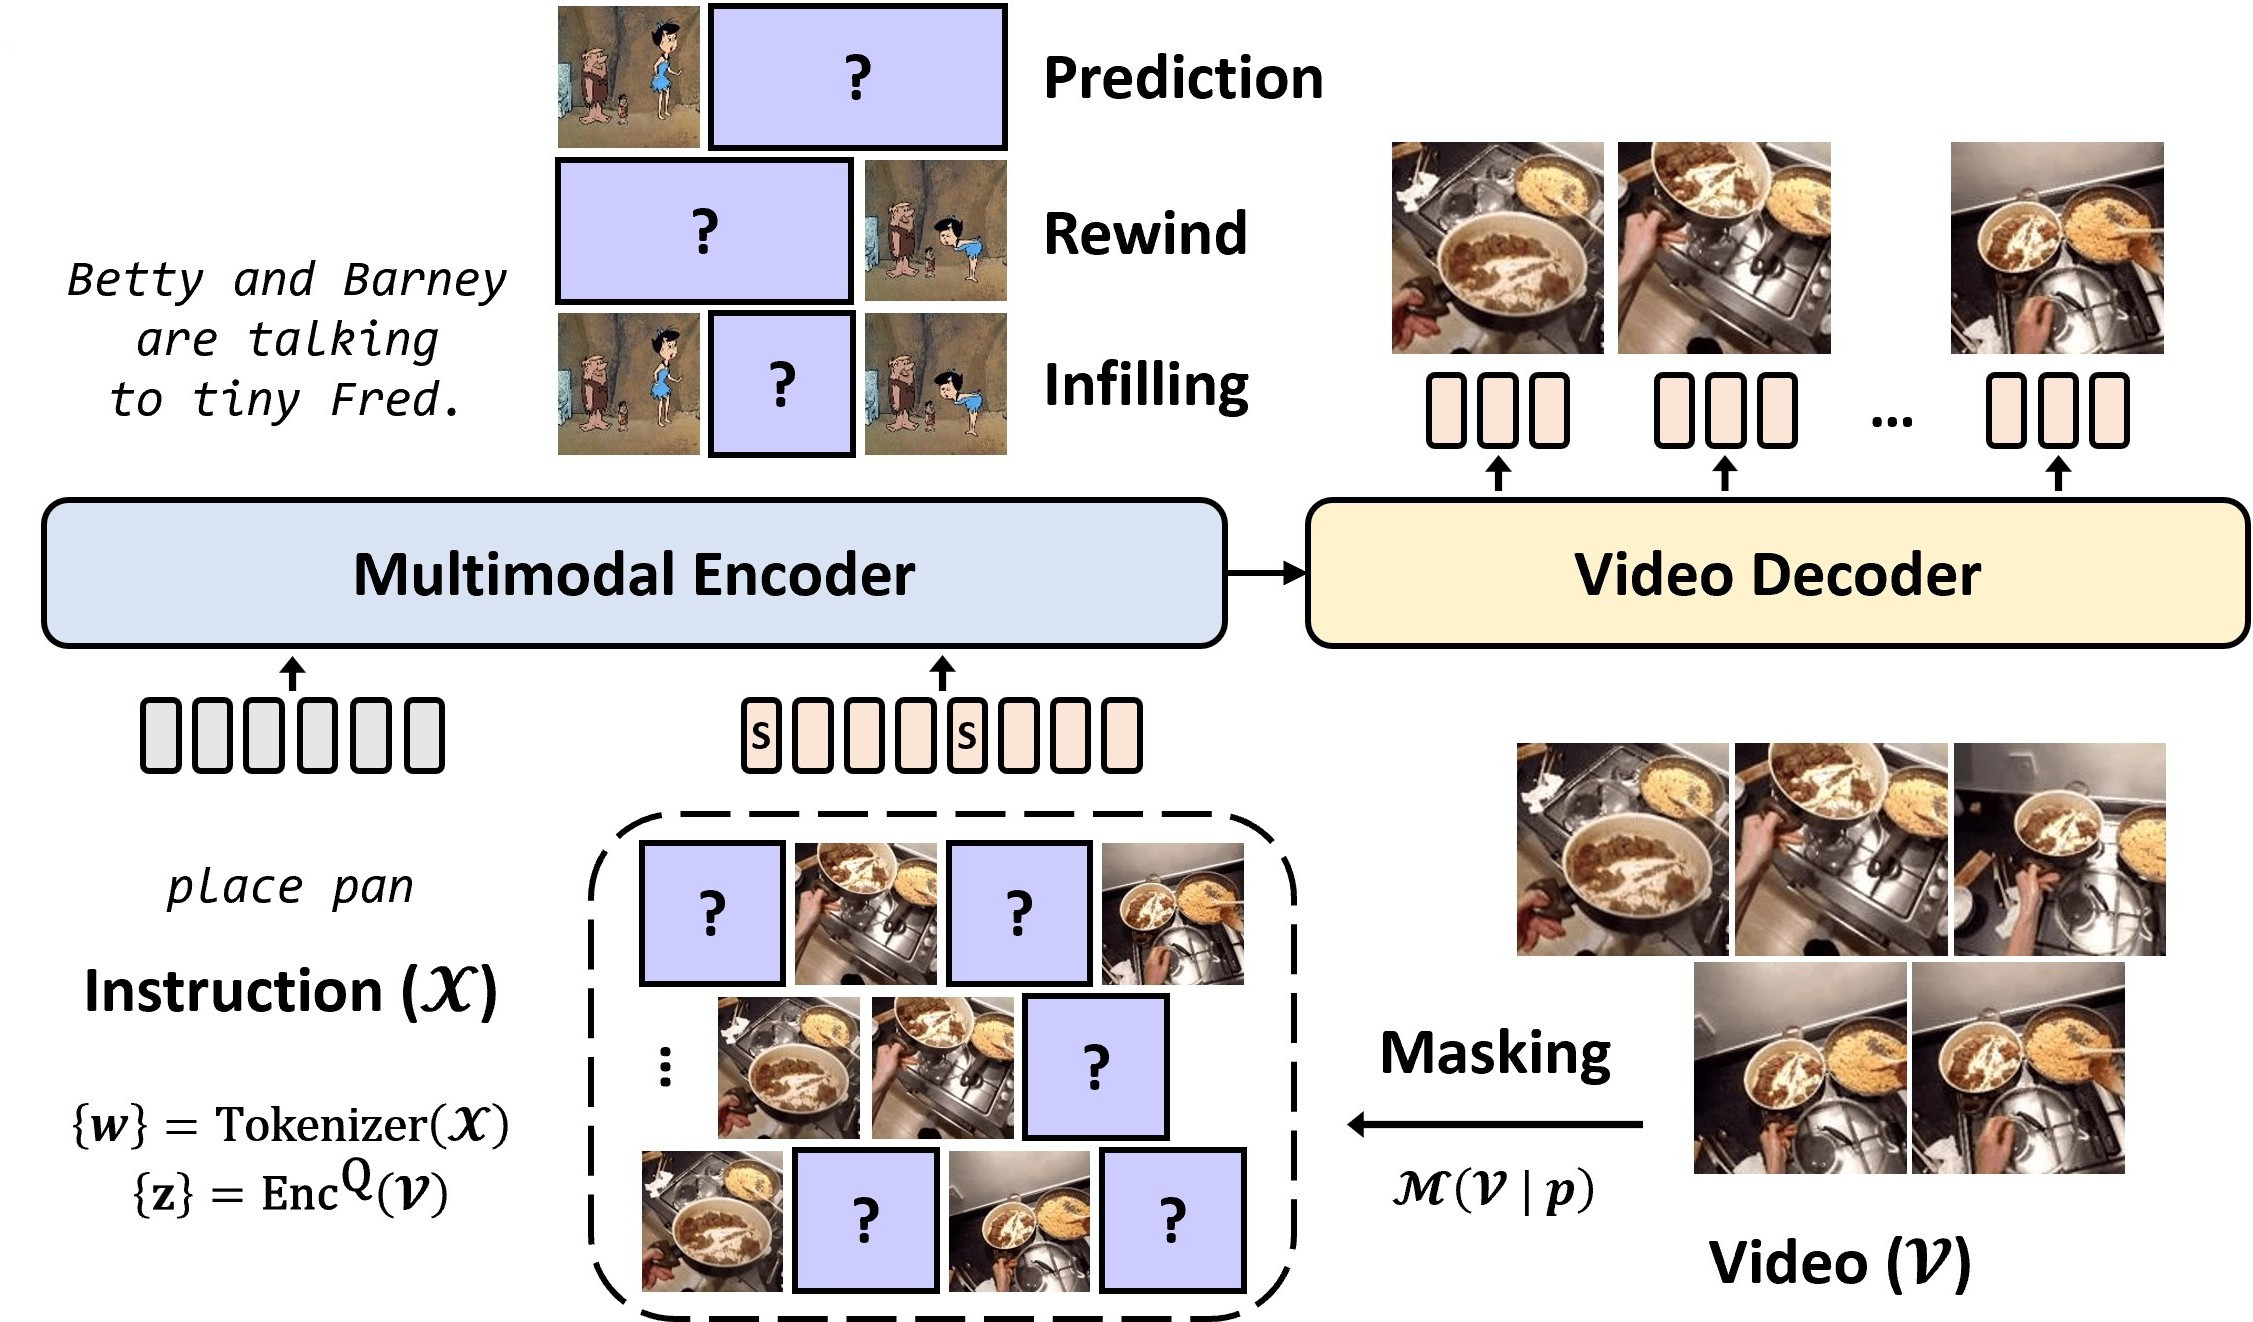
\includegraphics[width=\linewidth]{figs/fig_mmvg.jpg}
    \caption{\textbf{Multi-task video generation} model from \citet{fu2023tell}. Based on a partial video and a text prompt used to condition a codebook, a text-condition video VQGAN generates missing frames.}
    \label{fig:mmvg}
\end{figure}


\noindent
\textbf{Adversarially generated short video sequences}. Generative Adversarial Networks (GANs)~\citep{goodfellow2014generative} are based on an orthogonal objective between a generator network that synthesizes inputs from latent representations and a discriminator network optimized to distinguish between real and generated inputs. Video approaches extended the dimensionality of convolutional and deconvolutional kernels to space and time. An initial effort by \citet{vondrick2016generating} was to learn scene dynamics from unlabeled videos with a dual objective of generating static backgrounds and moving foregrounds. \citet{saito2017temporal} used a similar dual objective by first generating temporal adjacent views of latents and a spatial generator for frames. Works have also incorporated stochastic latent embeddings that can be decoded to the entire video \citep{lee2018stochastic}, separate spatial and temporal discriminators \citep{clark2019adversarial}, recurrent units \citep{gupta2022rv,wang2023styleinv}, and spatio-temporal kernel transformations \citep{luc2020transformation}. \citet{menapace2021playable} created an autoregressive approach to generate frames by conditioning the generation with discrete action labels. Other methods have adapted image-based GANs by generating latent trajectories of frame features \citep{tian2021good} or shifting frame features across time \citep{munoz2021temporal}. \citet{yu2022generating} used spatiotemporal coordinate information from latent representations of motion and video diversity. \citet{fu2023tell} used a variational-based GAN \citep{esser2021taming} to synthesize past or future frames (temporal outpainting) and current frames (inpainting) of videos based on both cues and textual descriptions. The model's pipeline is shown in \Cref{fig:mmvg}. A partial video is used alongside a codebook of latents to generate the remaining frames. Stop gradients are used to contrastively update the encoder and codebook. A final frame-wise feature-matching function is used to improve the embedding distance of embeddings from real and generated frames. 

%$\mathbf{v}$ with $\mathbf{T'}$ set of frames is used alongside a codebook of latents $\mathbf{C}$ to generate the remaining $\mathbf{T} \setminus \mathbf{T'}$ frames.
%\begin{equation}
%\begin{split}
%    \underset{VQ}{\mathcal{L}} = \underbrace{ \| \widehat{\mathbf{v}}_t - \mathbf{v}_t \|_1}_{\text{reconstr.}} + \underbrace{ \| \text{sg}[\mathcal{E}(\mathbf{v}_t)] - \mathbf{C}_{\mathbf{z}_t} \|_2^2}_{\text{code}}\\
%    + \underbrace{ \| \text{sg}[\mathbf{C}_{\mathbf{z}_t}] - \mathcal{E}(\mathbf{v}_t) \|_2^2}_{\text{commit}} + \underbrace{ \| \mathcal{F}(\widehat{\mathbf{v}}_t) - \mathcal{F}(\mathbf{v}_t) \|_1}_{\text{match}}
%\label{eq:vqae}
%\end{split}
%\end{equation}
%\noindent
%where $\mathcal{E}$ is the encoder, $\mathbf{z}_t$ are the codebook latents at time $t$ using quantizer $q$ and codebook $\mathbf{C}$, $\mathbf{z}_t=q(\mathcal{E}(\mathbf{v}_t)|\mathbf{C})$, and $\widehat{\mathbf{v}}=\mathcal{D}(\mathbf{z}_t)$ is the generated frame with decoder $\mathcal{D}$. 
% The generated frame index $t \in \mathbf{T} \setminus \mathbf{T}'$. 

Despite the progress in video generation by adversarial models, instability in training and mode collapse are the primary disadvantages of GANs that still present difficulties in generating realistic and diverse videos. 


\noindent
\textbf{Probabilistic models for video generation}. Denoising Diffusion Probabilistic Models (DDPMs) \citep{ho2020denoising,sohl2015deep,song2019generative} combine two Markov processes with the first (forward) corrupting the input data to noise within a distribution. The second (backward) process reverses this effect by reconstructing an input from the noisy representation. New inputs not in the training data are generated by sampling the prior distribution. \citet{ho2022video} directly extended this formulation to video by extending the original U-Net's \citep{salimans2017pixelcnn++} dimensionality used in the backward step with space-time kernels. Following works \citep{he2022latent,hong2022cogvideo,blattmann2023align} have moved away from pixel-level diffusion. They instead utilize the semantically rich and lower-dimensional latent space \citep{rombach2022high} with autoencoders to encode and project video inputs and outputs. The computational efficiency of Latent Diffusion Models (LDM) has enabled a new stream of works to improve temporal alignment of frames \citep{blattmann2023align,yang2023video} and minimize training data requirements \citep{nikankin2023sinfusion,wu2023tune}. \citet{yu2023avideo} combined the two approaches by projecting videos to triplane representations. \citet{yu2024efficient} adapted image-based models by incorporating low-resolution temporal content latents computed as the weighted sum of frames. Both image-based and low-resolution motion-based models are denoised with a similar training objective conditioned on the context vector. Although video context can improve frame generation, the number of frames these models can generate is still limited. 

%Given a video $\mathbf{v}$ of $T$ frames, a content frame $\overline{\textbf{v}}$ is computed as a weighted sum
%of frames. Given a context vector $\mathbf{c}$ that is associated with $\mathbf{v}$, the image-based denoising autoencoder model $\epsilon_I$ is fine-tuned based on:

%\begin{equation}   \underset{\overline{\textbf{v}}_0,\epsilon,t}{\mathbb{E}} \Bigl[ \| \epsilon - \epsilon_I(\overline{\textbf{v}}_t,\mathbf{c},t) \|_2^2 \Bigr] \; \text{where} \; \overline{\textbf{v}}_t \! = \! \sqrt{\overline{\alpha}_t}\overline{\textbf{v}}_0 \! +\! \sqrt{1-\overline{\alpha}}\epsilon 
%\label{eq:cmd_i}
%\end{equation}

%\noindent
%where $\overline{\alpha}$ are pre-defined hyperparameters. Similarly, the low-resolution motion-based model $\epsilon_V$ is optimized with a similar denoising training objective

%\begin{equation}   \underset{\textbf{z}_0,\epsilon,t}{\mathbb{E}} \Bigl[ \| \epsilon \! - \! \epsilon_V(\textbf{z}_t,\mathbf{c},\overline{\mathbf{v}},t) \|_2^2 \Bigr] \text{where} \; \textbf{z}_t \! = \! \sqrt{\overline{\alpha}_t}\textbf{z}_0 \! + \! \sqrt{1-\overline{\alpha}}\epsilon 
%\label{eq:cmd_v}
%\end{equation}

%\noindent
%where $\overline{\mathbf{z}}$ are latents from the entire video computed with ViViT \citep{arnab2021vivit}. 



\noindent
\textbf{Text-conditioned generation}. Language embeddings are increasingly used as a prior for video generation. The objective of these methods is to generate videos from textual descriptions based on visual-language correspondence. \citet{dorkenwald2021stochastic} used the start and end times as generation-controlling factors. 
Following methods explored T2V generation based on VQVAE codebooks conditioned on language \citep{han2022show,yan2021videogpt}, or language and motion \citep{hu2022make}. As LDM approaches rely on latent representations, unified visual-language embedding spaces can also be used to generate videos. LDM methods include joint conditional generation of images and videos \citep{gupta2023photorealistic}, shifting latent features for parameter-free temporal variance \citep{an2023latent}, and concatenating frames in spatial grids \citep{lee2024grid}. \citet{zeng2024make} showed that
first generating the start and end frames of the video to capture the start and end state enables models to effectively generate the transitioning frames limiting the dependence on well-formed textual descriptions. A number of recent works \citep{fei2024dysen,tian2024videotetris,wang2023videocomposer,wang2024recipe,wei2024dreamvideo,zhuang2024vlogger} have employed adapters on image-based LDMs similar to ControlNet's \citep{zhang2023adding} formulation. Given a pre-trained model using input latents and frozen parameters, a copy of the block is created with trainable parameters to adapt to a conditional latent. Condition latents can be of any modality type and are integrated into the frozen model with projection or cross-attention layers.

%\begin{equation}
%    \widehat{\mathbf{z}} = \mathcal{F}(\mathbf{z},\theta) + \mathcal{Z}_1(\mathcal{F}(\mathbf{z}+\mathcal{Z}_2(\mathbf{u},\vartheta_1),\vartheta),\vartheta_2)
%\end{equation}

%\noindent
%where $\widehat{\mathbf{z}}$ is the block's output and $\vartheta_1$ and $\vartheta_2$ are the learnable parameters for $\mathcal{Z}_1$ and $\mathcal{Z}_2$.


\noindent
\textbf{Generating long sequences}. Generating long videos is challenging as it requires models to learn long-range temporal dynamics. Initial efforts aimed to mitigate reductions in the generation quality over time through hybrid training schemes \citep{brooks2022generating} and by concatenating frame-wise codecs over time to allow frame consistency in generation \citep{skorokhodov2022stylegan}. \citet{shen2023mostgan} extended these approaches by using learnable latent vectors to represent motion styles and use them as priors to generate frames. \citet{harvey2022flexible} explored the conditionality between sampled frames for generating 25min videos with fixed backgrounds. A large number of approaches \citep{ho2022imagen,singer2023make} have focused on super-resolution models in tandem with LDMs to generate low-resolution long video sequences and then upsampling them to higher resolutions. Several models have been based on autoregression to accommodate for future unpredictability and large video changes. \citet{weissenborn2020scaling} extended the patch-based generation approach of Subscale Pixel Networks (SPNs)~\citep{menick2019generating} to spatio-temporal voxels. \citet{ge2022long} used an autoregressive transformer to generate latent representations for the next frames with a VQVAE as a backbone generator. Other auto-regressive VQVAE-based works explored dimension-specific \citep{wu2021godiva} and local attention \citep{liang2022nuwa,wu2022nuwa}. More recently, video generation methods have adapted causal attention encodings fused with previous frame features \citep{yan2023temporally,villegas2022phenaki}, or cross-attention adapters for fusing temporal context in image generators \citep{long2024videodrafter}, and guiding the generation with foreground masks \citep{chang2024look}.

%\begin{equation}
%    \underset{AT}{\mathcal{L}} = \underset{\mathbf{z} \sim p(\mathbf{Z})}{\mathbb{E}} \Bigl[ -\text{log} p(\mathbf{z}) \Bigr], \text{where} \; p(\mathbf{z}) = p(\mathbf{z}_0) \prod_{i=1}^{thw}  \underset{AT}{\Psi}(\mathbf{z}_{0:i})
%\end{equation}

%\noindent
%where $\mathbf{z}_0$ is the start of the sequence token. 


\subsubsection{Future outlooks}

Despite the recent substantial advancements of generative models, rudimentary challenges still exist that, in turn, provide opportunities for future approaches. Crucially, despite the high appearance quality of current models, a standardized \textbf{evaluation and benchmark method} is missing. Approaches based on T2V generation have been shown to replace concepts, fuse multiple concepts, or generate irrelevant objects using specific low-confidence prompts \citep{du2023stable}. The scope of current evaluation and benchmark methods \citep{huang2024vbench,liu2024evalcrafter,liu2023fetv,saito2020train,unterthiner2019fvd} is limited to primarily comparing the divergence of generated and real data distributions. Such comparisons do not reflect the extent to which the generated video conforms to the query, and how plausible the output is. The design of domain and characteristic-specific objectives is an interesting research direction. 

Another point of improvement for future works is the implementation of \textbf{generation control based on physical realism}. Although control of the generation process has been explored in many modalities \citep{zhang2023adding}, the number of works that aim to impose modality-specific characteristics and dynamics constraints in the generation remains small. Video consistency and physics failure cases highlighted in \Cref{fig:dlm_fails} can be addressed by conditional terms that provide implicit information about the visual world. Such information could also be used explicitly by relying on physics simulations that reason about physical objects in the scene \citep{liu2024physgen}.

The large capacity of generative models has shown great capabilities in simulating complex scenes. The impact of this has been shown in works that can simulate interactions of actors and objects both in the physical world \citep{yang2023learning} and visual virtually \citep{alonso2024diffusion,valevski2024diffusion}. Understanding parts of the world to generate video frames aligns with a number of downstream tasks that can enable \textbf{generative models to be used as general-purpose models}. 